\documentclass{article}

\usepackage[fontset = fandol]{ctex}
\usepackage{bm}
\usepackage{tikz}
\usepackage{float}
\usepackage[superscript]{cite}
\usepackage[table]{xcolor}
\usepackage{setspace}
\usepackage{datetime}
\usepackage{geometry}
\usepackage{graphicx}
\usepackage{enumitem}
\usepackage{listings}
\usepackage{booktabs}
\usepackage{pgfplots}
\usepackage{hyperref}
\usepackage{tcolorbox}
\usepackage{nicematrix}
\usepackage{amsmath, amssymb, amsfonts, mathrsfs}
\usepackage[fontsize = 12pt]{fontsize}

% \IfFontExistsTF{Times New Roman}{
%     \setmainfont{Times New Roman}
% }{
%     \setmainfont{TeX Gyre Termes
% }

\AtBeginDocument{
    \setlength{\abovedisplayskip}{4pt plus 2pt minus 2pt}
    \setlength{\belowdisplayskip}{4pt plus 2pt minus 2pt}
    \setlength{\abovedisplayshortskip}{4pt plus 1pt}
    \setlength{\belowdisplayshortskip}{4pt plus 1pt}
}

\pgfplotsset{compat = 1.18}
\usepgfplotslibrary{groupplots}
\usetikzlibrary{matrix, calc}

\newcommand{\diff}[2]{\dfrac{\mathrm{d}#1}{\mathrm{d}#2}}
\newcommand{\diffn}[3]{\dfrac{\mathrm{d}^{#3}#1}{\mathrm{d}#2^{#3}}}
\newcommand{\piff}[2]{\dfrac{\partial{#1}}{\partial{#2}}}
\newcommand{\eval}[2]{\left.#1\right|_{#2}}
\newcommand{\e}{\mathrm{e}}
\renewcommand{\d}{\mathrm{d}}
\newcommand{\barline}[1]{\overline{#1\rule{0pt}{1.5ex}}}
\newcommand{\norm}[1]{\left\lVert #1 \right\rVert}

\makeatletter
\renewcommand{\@citess}[1]{\textsuperscript{[#1]}}
\makeatother

\definecolor{Navy}{HTML}{16324F}
\definecolor{Wine}{HTML}{9A2E2E}
\definecolor{color1}{HTML}{EAE0D5}
\definecolor{color2}{HTML}{C6D5C5}
\definecolor{color3}{HTML}{82B0AA}
\definecolor{color4}{HTML}{4A8B93}
\definecolor{color5}{HTML}{00505F}
\definecolor{MorandiLightCyan}{RGB}{209, 238, 238}
\definecolor{MorandiBlue}{RGB}{70, 110, 255}
\definecolor{MorandiGrey}{RGB}{80, 100, 100}
\definecolor{MorandiPurple}{RGB}{140, 110, 180}
\definecolor{MorandiCyan}{RGB}{110, 170, 190}
\definecolor{MorandiRed}{RGB}{220, 130, 130}
\definecolor{MorandiOrange}{RGB}{250, 210, 160}

\newcommand{\cube}[1]{
    \begin{tikzpicture}[baseline = 0ex]
        \draw[
            draw = #1,
            fill = #1!20,
            thick,
            rounded corners = 0.5pt
        ] (0,0) rectangle (0.25, 0.25);
    \end{tikzpicture}
}

\pgfplotsset{
    swifftplot/.style = {
        tick label style = {font = \small},
        label style = {font = \small},
        title style = {font = \small\bfseries},
        legend style = {font = \small, draw = none},
        ymajorgrids = true,
        grid style = {dashed, color = black!18},
        axis line style = {black!50},
        tick style = {black!50}
    }
}

% \renewcommand{\thesubsection}{(\alph{subsection})}
\renewenvironment{abstract}{
    \begin{center}
        {\Large\bfseries \abstractname}
    \end{center}
    \quotation
}{\endquotation}

\geometry{
    a4paper,
    left = 1in,
    right = 1in,
    top = 1.25in,
    bottom = 1.25in
}

\hypersetup{
    colorlinks = true,
    linkcolor = Navy,
    citecolor = Wine,
    urlcolor = MorandiRed
}

\setlist[itemize,1]{
    itemsep = 2pt,
    partopsep = 0pt,
    parsep = \parskip,
    topsep = 5pt
}

\title{\bfseries\color[HTML]{16324F}从 Ring-SIS 到 SWIFFT：\\可证明安全 Hash 的 FFT 工程化}
\author{Illusionna · 2025............004 · 人工智能学院 · 计算机科学与技术}
\date{\currenttime,\ \today}



\begin{document}

\maketitle

\begin{abstract}
    后量子密码的工程应用不只包括密钥封装和数字签名，抗碰撞 Hash 函数同样是签名、承诺、认证数据结构和软件供应链完整性中的基础组件。本文以 SWIFFT 为核心案例，梳理一条从理论到工程的路线：SIS 可自然构造抗碰撞 Hash，Ring-SIS 将无结构矩阵压缩为环上卷积，SWIFFT 选择反循环环 $\mathbb{Z}_{257}[x]/(x^{64}+1)$，用有限域 FFT/NTT 将卷积变成逐点乘法，从而得到高并行、可证明安全的压缩函数。本文进一步给出碰撞到短关系的范数界、压缩率估算、负循环 NTT 公式和本机复现实验结果。实验部分报告 macOS Apple Sonoma M2 上吞吐、并行扩展、NEON 向量化收益和 Merkle 认证树演示，并明确区分原始压缩函数、工程封装与通用 Hash 的安全边界。
\end{abstract}

\noindent\textbf{关键词：}CRHF；理想格；Ring-SIS；FFT/NTT；SWIFFT；Merkle 树

\tableofcontents
% \clearpage



\section{引言}
NIST 后量子标准化让格密码最常以 ML-KEM/Kyber 和 ML-DSA/Dilithium 的形态出现，Falcon 也展示了基于 NTRU 格和快速傅里叶采样的签名路线~\cite{Kyber,Dilithium,Falcon}，但格密码并不只是 KEM 与签名，密码系统的安全性还依赖更底层的原语——\textbf{抗碰撞 Hash 函数}。数字签名需要先 Hash 消息，Merkle 树依赖 Hash 抗碰撞性，承诺方案和透明日志也需要将大对象压缩成不可伪造的短承诺。若量子计算威胁到整个密码栈，CRHF 也应有可证明后量子安全的候选，因此我们希望后量子安全覆盖整条密码链，而格密码恰好提供了一条独特路径：CRHF 的抗碰撞性可以归约到格上最坏情况困难问题，而不只是依赖“目前没有攻击”的经验信心~\cite{Ajtai96,LM06,PR06}。

SWIFFT 不是现实中替代 SHA-2/SHA-3 的通用 Hash 标准，而是具有工程价值的原型：它把 Ajtai 系列的 SIS/Ring-SIS 抗碰撞构造落到可运行代码中，并用 FFT 使理想格上的卷积计算接近工程可用~\cite{SWIFFT08,Repo}。
\[ \text{最坏情况格问题}\Longrightarrow\text{SIS}\Longrightarrow\text{CRHF}\Longrightarrow\text{Ring-SIS}\Longrightarrow\text{SWIFFT}\Longrightarrow\text{工程应用} \]

本文的目标不在于论述 SWIFFT 是否比 SHA-256 更安全更可靠，而是详细阐明以下四个核心问题：

\begin{itemize}
    \item[$\divideontimes$] SIS/Ring-SIS 为什么能产生抗碰撞 Hash？
    \item[$\divideontimes$] 为什么 SWIFFT 要选择 $x^{64}+1$ 和 $p=257$？
    \item[$\divideontimes$] FFT/NTT 在其中到底加速了什么？
    \item[$\divideontimes$] 它的工程价值和边界分别在哪里？
\end{itemize}



\section{相关工作}
SWIFFT 并不是孤立提出的工程 Hash 函数，而是建立在一系列关于格困难问题、紧凑表示和理想格构造的工作之上。本文将相关工作概括为四个层面：SIS 的理论基础、结构化 SIS 与紧凑 Hash、SWIFFT 的工程化实现，以及 SWIFFTX 对通用 Hash 场景的进一步扩展。

SIS 与最坏情况格困难性，Ajtai 关于随机格问题与最坏情况格问题之间联系的开创性工作，为后续基于格的单向函数和抗碰撞 Hash 奠定了理论基础~\cite{Ajtai96}。SIS 小整数解问题核心形式是从给定的均匀随机矩阵 $\bm{A}\in\mathbb{Z}_{q}^{n\times m}$ 中寻找非零整型短向量 $\bm{v}$，满足：
\[ \bm{A}\bm{v}\equiv\bm{0}\pmod q\qquad\|\bm{v}\|\leqslant\beta \]

这一问题天然适合构造压缩函数，因为一旦两个不同输入在映射 $\bm{x}\mapsto \bm{A}\bm{x}\bmod q$ 下发生碰撞，其差值便给出一个短的 SIS 解。因此，SIS 成为格密码中连接“平均情形实例”和“抗碰撞 Hash 构造”的基本桥梁。

SIS 构造虽然理论清晰，但需要存储和计算大规模随机矩阵，工程效率较低。Micciancio 提出的 Generalized Compact Knapsack 将线性映射结构化到循环格或理想格相关的代数对象中，使得矩阵可以由少量环元素紧凑表示，多项式乘法也可以替代一般矩阵乘法~\cite{Micciancio07}。这一思想显著改善了存储和计算效率，但也引入新的代数结构，因此不能简单地把 SIS 的安全直觉无条件迁移到结构化情形中。特别地，朴素循环环 $\mathbb{Z}[x]/(x^n-1)$ 在二进制 Compact Hash 设计中会产生全一向量导致的结构性碰撞，这说明环的选择本身是安全设计的一部分，而不仅是实现细节~\cite{LM06,PR06}。

抗碰撞 Compact Hash 与理想格路线在这样的背景下应运而生。文献~\cite{LM06,PR06} 进一步发展了基于 Compact Knapsack、循环格的抗碰撞 Hash 构造，系统说明了如何在保持紧凑表示和高效计算的同时获得抗碰撞性。这些工作的重要意义在于，不只是提出一个具体的函数，而是将“寻找碰撞”与“求解结构化格中的短关系”联系起来，从而把 Hash 的安全性建立在理想格相关的最坏情况困难假设之上，而 SWIFFT 正是这一理论路线的一个具体实例化~\cite{SWIFFT08}。

SWIFFT 将上述思想具体落实为参数 $n=64$、$m=16$、$p=257$ 的压缩函数，工作在反循环环之上：
\[ \mathbb{Z}_{257}[x]/(x^{64}+1) \]

它利用模 257 的有限域 FFT/NTT 将环上卷积转化为频域逐点乘法，从而兼具紧凑密钥、高并行性和较好的软件实现效率~\cite{SWIFFT08,Repo}。SWIFFT 的贡献并不只是在 Hash 中使用 FFT，而是在抗碰撞 Hash 这一基础原语中展现的可证明安全、代数结构和工程优化之间的结合。SWIFFT 本身是线性压缩函数，线性性质有助于建立清晰的碰撞归约，但也限制了它作为通用 Hash 的适用范围，它不能直接被当作随机 Oracle、PRF 或 SHA-3 风格的通用摘要函数。

SWIFFTX 作为后续 SHA-3 候选方案，在 SWIFFT 的基础上加入非线性层、填充规则和更完整的 Hash 封装，试图弥补线性压缩函数在通用应用中的不足~\cite{SWIFFTX}。本文的重点仍放在 SWIFFT 本身，SWIFFTX 主要用于说明其应用边界与可能扩展方向。

综上，本文不仅复述 SWIFFT 论文，而且也围绕“从 Ring-SIS 到 FFT 工程化”这一主线，连接 SIS、Ring-SIS、理想格、卷积计算和 NTT 实现，接下来的报告特别区分严格安全归约、具体参数安全性和工程演示结果，避免将“压缩函数”、“任意长 Hash”、“随机 Oracle 机式通用 Hash”混为一谈。



\section{从 SIS 到抗碰撞 Hash}
SIS 问题的定义是，给定均匀随机矩阵 $\bm{A}\in\mathbb{Z}_{q}^{n\times m}$ 与界 $\beta$，小整数解问题 $\operatorname{SIS}_{n,m,q,\beta}$ 要求找到非零短向量 $\bm{v}\in\mathbb{Z}^{m}$，使得：
\[ \bm{A}\bm{v}\equiv\bm{0}\pmod q\qquad 0<\|\bm{v}\|\leqslant\beta \]

通常地，“短”通常指 $\ell_2$ 范数或 $\ell_{\infty}$ 范数受限，SIS 与 Hash 的关系非常直接，定义：
\[ h_{\bm{A}}:\ \{0,1\}^{m}\to\mathbb{Z}_{q}^{n}\qquad h_{\bm{A}}(\bm{x})=\bm{A}\bm{x}\bmod q \]

当 $2^{m}>q^{n}$ 时，定义域大于值域，因此它是压缩函数，更具体地说，平均每个输出对应若干个输入前像：
\[ \dfrac{2^m}{q^n}=2^{m-n\log_2q} \]

若攻击者找到碰撞 $h_{\bm{A}}(x)=h_{\bm{A}}(x')$，则：
\[ \bm{A}(\bm{x}-\bm{x}')\equiv\bm{0}\pmod q \]

且 $\bm{x}-\bm{x}'\in\{-1,0,1\}^{m}\backslash\{0\}$，令 $\bm{v}=\bm{x}-\bm{x}'$，则：
\[ \norm{\bm{v}}_\infty\leqslant1,\qquad\norm{\bm{v}}_2\leqslant\sqrt{m} \]

于是碰撞直接给出一个短 SIS 解，所以给出最核心的安全逻辑：
\[ \text{找 Hash 碰撞}\quad\Longrightarrow\quad\text{解 SIS} \]

Ajtai 的最坏情况到平均情况归约说明，适当参数下随机 SIS 实例的困难性可由最坏情况格问题支撑~\cite{Ajtai96}，这让 SIS Hash 与传统经验型 Hash 的哲学不同：它不是只说目前没有攻击，而是把碰撞困难性和格问题困难性联系起来。无结构 SIS 的缺点也明显，矩阵 $\bm{A}$ 大，矩阵向量乘法代价高，若 $\bm{A}$ 是一般稠密矩阵，密钥存储需要 $nm\log_2q$ bit，单次计算也需要约 $nm$ 次模乘加，很难与 SHA 系列竞争，Ring-SIS 的引入就是为了用代数结构压缩矩阵并加速乘法。



\section{Ring-SIS}
令：
\[ R=\mathbb{Z}[x]/\left(f(x)\right)\qquad R_q=R/qR \]

环元素可视为长度为 $n=\deg f$ 的系数向量，用一个环元素 $a$ 乘以另一个环元素 $z$，等价于用一个由 $a$ 决定的结构化矩阵乘以 $z$ 的系数向量，于是 SIS 的矩阵列可以被环元素的“乘法矩阵”替代。

以 $R_q=\mathbb{Z}_q[x]/(x^n+1)$ 为例，若 $a(x)=a_0+a_1x+\cdots+a_{n-1}x^{n-1}$，则 $a(x)z(x)\bmod(x^n+1)$ 对应的负循环矩阵形如：
\[ M_a=\begin{pmatrix}
    a_0      & -a_{n-1} & -a_{n-2} & \cdots & -a_1\\
    a_1      & a_0      & -a_{n-1} & \cdots & -a_2\\
    \vdots   & \vdots   & \vdots   & \ddots & \vdots\\
    a_{n-2}  & a_{n-3}  & a_{n-4}  & \cdots & -a_{n-1}\\
    a_{n-1}  & a_{n-2}  & a_{n-3}  & \cdots & a_0 \\
\end{pmatrix} \]

因此，一个环元素 $a$ 就隐式表示了 $n\times n$ 个矩阵项，紧凑性来自这种代数结构。Ring-SIS 问题的定义是，给定 $a_1,a_2,\ldots,a_m\in R_q$ 与短向量界 $\beta$，Ring-SIS 要求找到非零短元素组 $z_1,z_2,\ldots,z_m\in R$，使：
\[ \sum_{i=1}^{m}a_iz_i\equiv0\pmod q \]

相应的 Ring-SIS Hash 写作：
\[ h_{\bm{a}}(z_1,z_2,\ldots,z_m)=\sum_{i=1}^{m}a_iz_i\pmod q\qquad z_i\in\{0,1\}^{n} \]

如果有碰撞 $h_{\bm{a}}(z)=h_{\bm{a}}(z')$，则：
\[ \sum_{i=1}^{m}a_i(z_i-z_i')\equiv0\pmod q \]

并且 $z_i-z_i'\in\{-1,0,1\}^n$，因此碰撞仍然给出 Ring-SIS 短解。Ring-SIS 的工程收益也很直接，无结构 SIS 需要存储大矩阵，Ring-SIS 只需存储若干环元素，乘法也从一般矩阵乘法变成环上多项式卷积，而卷积可以用 FFT/NTT 加速。

\begin{table}[H]
    \centering
    \renewcommand{\arraystretch}{1.5}
    \setlength{\tabcolsep}{16pt}
    \caption{SIS Hash 与 Ring-SIS Hash 的对比}
    \begin{tabular}{ccc}
        \toprule[1.5pt]
        维度 & SIS Hash & Ring-SIS/SWIFFT 路线 \\
        \midrule[0.75pt]
        代数对象 & 矩阵 $\bm{A}\in\mathbb{Z}_{q}^{n\times m}$ & 环 $R_q=\mathbb{Z}_q[x]/(f)$ 上的元素 \\
        核心运算 & 矩阵向量乘法 & 多项式卷积 \\
        密钥规模 & 大矩阵 & 若干紧凑的多项式 \\
        加速方式 & 一般线性代数优化 & FFT/NTT \\
        安全假设 & 一般格 SIS & 理想格/结构化 Ring-SIS \\
        \bottomrule[1.5pt]
    \end{tabular}
\end{table}

代价也同样清楚，Ring-SIS 引入结构后，安全假设比 SIS 更强、更具体，但不能只考虑速度更快，还必须有结构化带来的攻击面。



\section{SWIFFT 压缩函数}
SWIFFT 可抽象为公开随机密钥下的环上线性压缩函数，其核心参数为~\cite{SWIFFT08}：
\[ n=64\qquad m=16\qquad p=257\qquad R_p=\mathbb{Z}_{257}[x]/(x^{64}+1) \]

输入是 $m=16$ 个二进制多项式 $x_i\in\{0,1\}^{64}$，总输入长度为 1024bit，密钥为 $a_1,a_2,\ldots,a_{16}\in R_p$，数学上可理解为：
\[ H_{\bm{a}}:\left(\{0,1\}^{64}\right)^{16}\longrightarrow R_p,\qquad H_{\bm{a}}(x_1,x_2,\ldots,x_{16})=\sum_{i=1}^{16}a_ix_i\pmod p \]

Micciancio 的 SWIFFT 实现中包含居中表示和常数校正项，但这些项在碰撞差分中会抵消，不改变“碰撞推出 Ring-SIS 解”的核心关系，输出属性 $R_p$，即 64 个模 257 的系数，其信息量约为：
\[ 64\log_{2}257\approx512.36\ \text{bit} \]

所以该压缩函数的平均压缩量为：
\[ \log_2\dfrac{2^{1024}}{257^{64}}=1024-64\log_2 257 \approx511.64\ \text{bit} \]

换言之，平均每个输出约对应 $2^{511.64}$ 个输入前像，这是抗碰撞问题必须依赖计算困难性而非单射性的原因，若 $x\neq x'$ 发生碰撞，令 $z_i=x_i-x_i'$，则每个差分多项式满足：
\[ z_i\in\{-1,0,1\}^{64},\qquad\sum_{i=1}^{16}\norm{z_i}_2^2\leqslant16\times64=1024 \]

因此碰撞给出的 Ring-SIS 解满足 $\norm{z}_2\leqslant32$ 且 $\norm{z}_\infty\leqslant1$，将每个输出系数的低 8 位和第 9 位分开存储，参考代码得到 72 字节编码，若使用紧凑 base-257 编码，则约 513 bit 足够。与此同时，这组参数也揭示了 SWIFFT 的权衡：全部运算都是线性的，因此碰撞和 Ring-SIS 解之间关系清晰，但也正因为线性，它不是随机 Oracle 式的 Hash。



\section{FFT/NTT 变换}
在 $R_p=\mathbb{Z}_{p}[x]/(x^{n}+1)$ 中，乘法是负循环卷积，若 $\omega$ 是模 $p$ 下的 $2n$ 次本原单位根，则 $x^{n}+1$ 的根是：
\[ \omega^{2j+1}\qquad j=0,1,\ldots,n-1 \]

因此可定义变换：
\[ \widehat{x}_j=\sum_{k=0}^{n-1}x_k\omega^{(2j+1)k}\pmod p \]

在这个频域内进行卷积变逐点乘法：
\[ \widehat{a\cdot x}_j=\widehat a_j\widehat x_j \]

此时逆变换可写成：
\[ x_k=n^{-1}\sum_{j=0}^{n-1}\widehat{x}_j\omega^{-(2j+1)k}\pmod p \]

其中 $n^{-1}$ 是 $n$ 在 $\mathbb{Z}_p$ 中的乘法逆元，SWIFFT 取 $n=64$，因此需要 $2n=128$ 次单位根，素数：
\[ p=257=2^8+1\qquad p-1=256 \]

满足整除 $128\mid 256$，所以模 257 下存在 128 次本原单位根，参考实现中使用的根为 $\omega=42$，它满足 $42^{128}\equiv1\pmod{257}$ 且 $42^{64}\equiv-1\pmod{257}$~\cite{Repo}。此外，$257$ 接近一个字节的范围，使查表和 SIMD 实现都很自然。Micciancio 代码还利用输入为二进制这一事实，每 8 位分成一个小块，预先把 $2^8$ 种可能的局部 FFT 结果存入表中，这样扩散层可以大量通过查表完成，而不是运行一般的复杂 FFT，实现了预计算。

从算法复杂度来看，若直接计算 $16$ 个长度 $64$ 的负循环卷积，朴素方法所需系数级乘加约：
\[ C_{\text{naive}}\asymp m n^2=16\cdot64^2=65536 \]

若密钥预先保存在频域，则在线阶段主要是输入变换、逐点乘法和求和：
\[ C_{\text{NTT}}\asymp m n\log_2n+mn \]

而 SWIFFT 的二进制查表进一步把输入变换中的大量固定线性组合折叠进预计算表，这里 FFT/NTT 加速的不是 Hash 的“随机性”，而是 $R_p$ 上的多项式乘法。

\begin{table}[H]
    \centering
    \renewcommand{\arraystretch}{1.5}
    \setlength{\tabcolsep}{16pt}
    \caption{SWIFFT 参数与编码}
    \begin{tabular}{cccc}
        \toprule[1.5pt]
        参数 & 数值 & 作用 & 工程含义 \\
        \midrule[0.75pt]
        $n$ & 64 & 环维数 & 每块 64 bit，NTT 长度 64 \\
        $m$ & 16 & 输入块数 & 总输入 1024 bit \\
        $p$ & 257 & 模数 & $128\mid p-1$，支持负循环 NTT \\
        $\omega$ & 42 & $2n$ 次单位根 & 参考实现常量 \\
        输出值域 & $257^{64}$ & 约 512.36 bit & 代码编码为 72 字节 \\
        \bottomrule[1.5pt]
    \end{tabular}
\end{table}



\section{安全性边界}
SWIFFT 的抗碰撞证明可以分成两层，代数层和困难性层。第一层是代数层，若输入 $x\neq x'$ 产生碰撞，则：
\[ \sum_{i}a_i(x_i-x_i')\equiv0\pmod p \]

其中每个 $x_i-x_i'$ 的系数属于 $\{-1,0,1\}$，这就是一个短 Ring-SIS 解。第二层是困难性层，SWIFFT 相关论文把这类随机 Ring-SIS/Compact Knapsack 问题与某些理想格上的最坏情况短向量问题联系起来，因此，随机密钥下找碰撞的算法可转化为求解相应结构化格问题的算法~\cite{LM06,PR06,SWIFFT08}。忽略归约损耗时，可以把这层关系概括为：
\[ \operatorname{Adv}^{\mathrm{cr}}_{H_{\bm a}}(\mathcal{A})\lesssim\operatorname{Adv}^{\mathrm{rsis}}_{n,m,p,\beta}(\mathcal{B})\qquad\beta\approx32 \]

这里左边是攻击者 $\mathcal{A}$ 找到 SWIFFT 碰撞的优势，右边是由 $\mathcal{A}$ 构造出的算法 $\mathcal{B}$ 求解相应 Ring-SIS 短关系的优势。

因此，我们给出了“可证明安全”的意义，但不可认为成“任何具体参数都等于 256 bit 安全”。由于 SWIFFT 的输出值域约 512 bit，并不意味着碰撞复杂度就是 $2^{256}$，具体参数需要考虑 Generalized Birthday Attacks 和格约化攻击~\cite{Wagner02,SWIFFT08}。SWIFFT 展示了可证明安全与高效实现的结合，但其原始参数不是面向现代 128/256 bit 通用 Hash 安全级别的最终标准。

SWIFFT 是线性压缩函数，线性性让碰撞自然变成 Ring-SIS 短解，这是安全归约的根，线性性也意味着它不能直接作为随机 Oracle、PRF 或 SHA-3 风格通用 Hash 使用，需要随机 Oracle 性质或通用摘要接口时，应考虑 SWIFFTX 等加入非线性层的后续设计~\cite{SWIFFTX}。我们可以把 SWIFFT 安全证明逻辑拆分成三步：

\begin{itemize}
    \item[$\divideontimes$] 碰撞到短关系。给定同一个公开密钥 $\bm{a}=(a_1,a_2,\ldots,a_m)$，若 $x\neq x'$ 且需要满足 $H_{\bm{a}}(x)=H_{\bm{a}}(x')$，让 $z_i=x_i-x_i'$，由于输入块是二进制，$z_i$ 的系数落在 $\{-1,0,1\}$，碰撞等价于 $\displaystyle\sum_{i}a_iz_i\equiv0\pmod p$，因此 $z=(z_1,z_2,\ldots,z_m)$ 是一个短关系。
    \item[$\divideontimes$] 短关系到 Ring-SIS。上式正是 $R_p=\mathbb{Z}_{257}[x]/(x^{64}+1)$ 上的 Ring-SIS 解，这里的短关系是由差分系数属于 $\{-1,0,1\}$ 给出明确范数界。
    \item[$\divideontimes$] 平均情况到最坏情况。相关理论工作说明，随机选择的 $a_i$ 上求这种短关系，与某些理想格类上的最坏情况短向量问题相联系，Ring-SIS 的困难性有最坏情况理想格问题作为支撑，这种渐近归约和结构化假设不是对任意参数的无条件安全证明。
\end{itemize}



\section{实验方法的工程实现}
Micciancio 的 GitHub 仓库 SWIFFT 代码明确指出：它基本是 2007 年用于论文测试的原始代码，面向当时 32-bit Intel CPU 与 SSE 指令集优化，代码主要用于复现和测试，并不包含完整任意长 Hash，只实现固定长度压缩函数~\cite{Repo}，其接口可概括为：
\[ \text{SWIFFT}(\text{key},\text{state},\text{data}) \]

其中 state 为 72 字节，data 为 56 字节，合计 128 字节输入，输出更新为新的 72 字节 state，为了做工程演示，我们在实验代码外层加上：

\begin{itemize}
    \item 一个 Merkle--Damg\aa rd 风格的任意长吸收过程，每次吸收 56 字节；
    \item 一个 Merkle 树封装，用完整 72 字节 SWIFFT 状态作为叶子和内部节点摘要；
    \item 一个逐坐标标量版本与参考向量版本的对比，用于测量显式 SIMD 向量类型收益。
\end{itemize}

实验中的 Merkle 演示保留完整 72 字节状态，避免把截断摘要误写成原论文定理的直接对象，任意长吸收和 Merkle 域分离是本文实验代码中的工程封装，不等同于 SWIFFTX 的正式通用 Hash 规范。

本次复现实验环境为 macOS Sonoma Apple M2 clang 16.0.0，SWIFFT benchmark 使用 \texttt{-O3}、\texttt{-funroll-loops}、\texttt{-fno-vectorize} 和 \texttt{-fno-slp-vectorize} 编译，以关闭普通 C 循环的自动向量化，同时保留原始 \texttt{ZW} 显式向量类型在 arm64 上生成的 NEON 指令，SHA 对照使用同一环境中的 OpenSSL 3.0.15~\cite{OpenSSL}，计时口径如下：
\[ \text{吞吐}=\frac{\text{处理的消息字节数}}{\text{总耗时}}\qquad\text{单次延迟}=\frac{1}{\text{压缩函数调用次数}/\text{秒}} \]

多线程实验使用独立消息流消除跨线程依赖，标量与向量版本在 10000 组随机输入上逐字节比对输出，确认优化不改变函数语义，除 Merkle 建树外，SWIFFT 数字均取 7 次重复的中位数。由于桌面后台负载会影响计时，本文使用“约值”和同量级比较，不把单次数字解释为基准排名。



\section{实验结果}
\subsection{吞吐与 SHA 对比}
本次实验中，SWIFFT 原始压缩函数中位数为 4.25 Mops/s，单次压缩约 235 ns。若按压缩函数完整 128 字节输入计，等效吞吐为 544 MB/s，若按外层 MD 每次实际吸收的 56 字节消息，应用侧吞吐为 238 MB/s。对照组中，OpenSSL SHA-256 为 2540 MB/s，SHA3-256 为 672 MB/s。

\begin{table}[H]
    \centering
    \renewcommand{\arraystretch}{1.5}
    \setlength{\tabcolsep}{12pt}
    \caption{macOS Sonoma Apple M2 clang 16.0.0 上的单核吞吐对比}
    \begin{tabular}{clcc}
        \toprule[1.5pt]
        ~ & \textbf{方案} & \textbf{吞吐} & \textbf{说明} \\
        \midrule[0.75pt]
        \cube{MorandiBlue} & SWIFFT 压缩函数 & 4.25 Mops/s & 每次 128B 输入、72B 状态输出 \\
        \cube{MorandiCyan} & SWIFFT 压缩函数 & 544 MB/s & 按 128B 压缩块折算 \\
        \rowcolor{MorandiLightCyan}\cube{MorandiPurple} & SWIFFT-MD & 238 MB/s & 每次吸收 56B 数据 \\
        \cube{MorandiRed} & OpenSSL SHA-256 & 2540 MB/s & OpenSSL 3.0.15 EVP/speed \\
        \cube{MorandiOrange} & OpenSSL SHA3-256 & 672 MB/s & OpenSSL 3.0.15 EVP/speed \\
        \bottomrule[1.5pt]
    \end{tabular}
\end{table}

\begin{figure}[H]
    \centering
    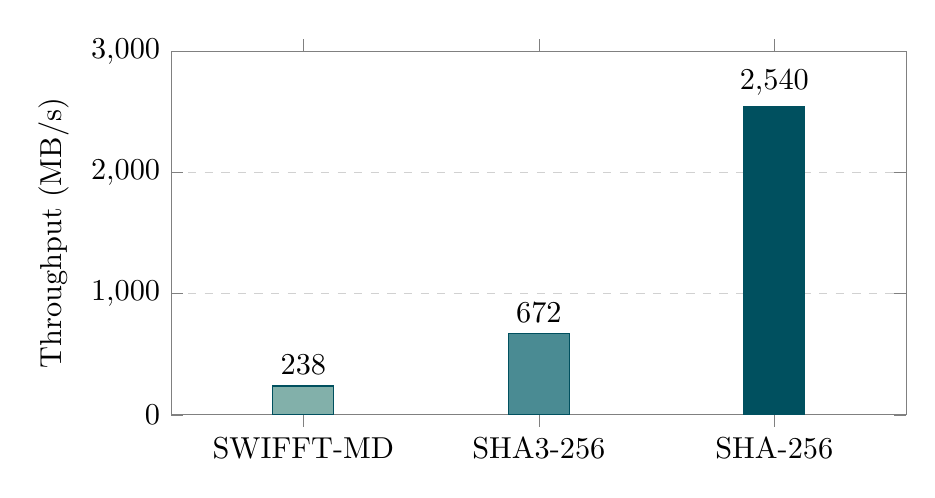
\begin{tikzpicture}
        \begin{axis}[
            swifftplot,
            ybar = 0pt,
            width = 0.9\linewidth,
            height = 6.2cm,
            ymin = 0,
            ymax = 3000,
            ylabel = {Throughput (MB/s)},
            symbolic x coords = {SWIFFT-MD, SHA3-256, SHA-256},
            xtick = {SWIFFT-MD, SHA3-256, SHA-256},
            bar shift = 0pt,
            enlarge x limits = 0.28,
            /pgf/bar width = 22pt,
            nodes near coords,
            nodes near coords style = {font = \small, anchor = south},
            tick label style = {font = \small},
            x tick label style = {align = center}
        ]
            \addplot[fill = color3, draw = color5] coordinates {(SWIFFT-MD, 238)};
            \addplot[fill = color4, draw = color5] coordinates {(SHA3-256, 672)};
            \addplot[fill = color5, draw = color5] coordinates {(SHA-256, 2540)};
        \end{axis}
    \end{tikzpicture}
    \caption{SWIFFT-MD 按每次吸收 56 字节消息，OpenSSL speed 按 1MiB 块测试}
\end{figure}

值得注意的是，实验结果不能简单解读为 SWIFFT 没有工程价值，SHA-256 在 M2 上享有专用加密指令，而 SWIFFT 使用通用 SIMD，更合理的是，原始 SWIFFT 参考实现作为 2007 年代码已经能达到数百 MB/s 量级，但若要和现代 SHA 实现比裸吞吐，需要重新做 AVX2/AVX-512/NEON/SVE 级别的工程优化。



\subsection{并行扩展}
SWIFFT 的结构非常适合并行，不同块的 FFT、不同消息流、不同树节点都可独立计算。我们在本节用加速比 $S_t$ 和并行效率 $\eta_t$ 描述扩展性：
\[ S_t=\dfrac{T_t}{T_1}\qquad\eta_t=\frac{T_t}{tT_1} \]

其中 $T_t$ 是 $t$ 个线程下的总吞吐，本次实验中 SWIFFT-MD 多线程扩展曲线如下：

\begin{figure}[H]
    \centering
    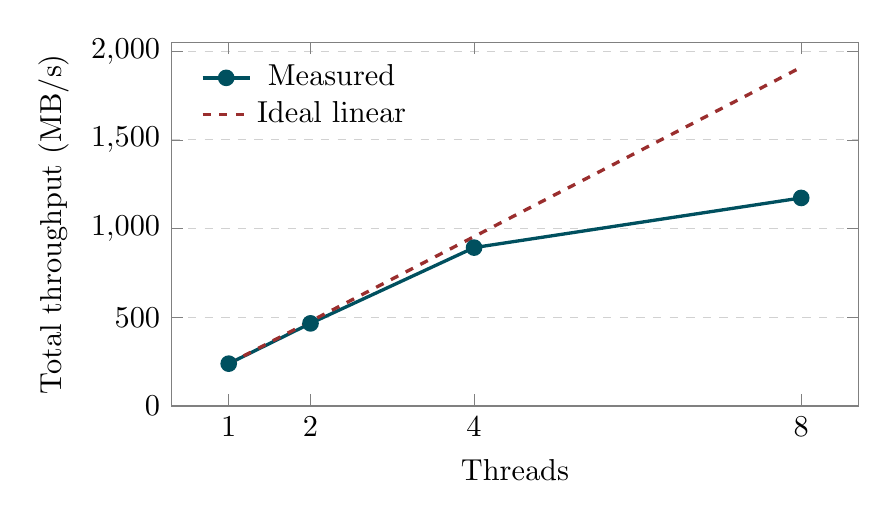
\begin{tikzpicture}
        \begin{axis}[
            swifftplot,
            width = 0.85\linewidth,
            height = 6.2cm,
            xlabel = {Threads},
            ylabel = {Total throughput (MB/s)},
            xtick = {1, 2, 4, 8},
            ymin = 0,
            ymax = 2050,
            legend pos = north west
        ]
            \addplot[
                mark = *,
                mark size = 2.4pt,
                very thick,
                color = color5
            ] coordinates {(1, 238.72) (2, 465.83) (4, 892.87) (8, 1172.95)};
            \addlegendentry{Measured}
            \addplot[
                dashed,
                very thick,
                color = Wine
            ] coordinates {(1, 238.72) (2, 477.44) (4, 954.89) (8, 1909.77)};
            \addlegendentry{Ideal linear}
        \end{axis}
    \end{tikzpicture}
    \caption{线程为 4 个时呈现近线性，线程为 8 个时受能效核、调度和内存层次影响}
\end{figure}

由图中数据可得，1、2、4、8 线程的总吞吐分别约为 239、466、893、1173 MB/s，2 线程并行效率约为 $97.6\%$，4 线程约为 $93.5\%$，8 线程降至约 $61.4\%$，这说明 SWIFFT 的核心运算具备并行性，但真实机器上仍受核心异构、调度和内存层次影响。



\subsection{NEON 向量化收益}
参考实现使用 GCC 向量类型描述 8 路 16-bit 并行数据，在 arm64 上，clang 会把这些显式向量操作编译成 NEON 指令。为了量化这一点，实验代码写了一个逐坐标标量版本，并在编译时关闭自动向量化，该标量版本与参考版本逐字节比对 10000 组随机输入，结果完全一致：

\begin{table}[H]
    \centering
    \renewcommand{\arraystretch}{1.5}
    \setlength{\tabcolsep}{22pt}
    \caption{标量基线与显式 NEON/SIMD 向量实现对比}
    \begin{tabular}{cccc}
        \toprule[1.5pt]
        & \textbf{版本} & \textbf{吞吐} & \textbf{相对标量加速} \\
        \midrule[0.75pt]
        \cube{MorandiGrey} & 纯标量基线 & 30.2 MB/s & 1.00x \\
        \rowcolor{MorandiLightCyan}\cube{MorandiBlue} & 显式向量实现 & 238.1 MB/s & 7.89x \\
        \bottomrule[1.5pt]
    \end{tabular}
\end{table}

这表明 SWIFFT 的 FFT 线性组合结构确实适合 SIMD，进一步提速不应只是把 C 改写成 intrinsics，而应考虑数据布局、批量消息、多路树节点和更宽向量指令。



\subsection{Merkle 认证树演示}
实验还把 SWIFFT 封装成 Merkle 认证树，用于演示抗碰撞 Hash 的应用形态，若叶子数为 $N=2^h$、节点摘要长度为 $d$ 字节，则一条认证路径大小为：
\[ |\pi|=h\cdot d \]

表中的实现使用完整 72 字节状态，因此 $d=72$，但此处仍是工程演示，严格通用 Hash 构造应使用正式填充、域分离和安全证明完整的封装。

\begin{table}[H]
    \centering
    \renewcommand{\arraystretch}{1.5}
    \setlength{\tabcolsep}{12pt}
    \caption{SWIFFT-MD 封装下的 Merkle 认证树演示}
    \begin{tabular}{ccccccc}
        \toprule[1.5pt]
        & \textbf{叶子数} & \textbf{树高} & \textbf{建树时间} & \textbf{证明大小} & \textbf{验证时间} & \textbf{篡改检测} \\
        \midrule[0.75pt]
        \cube{MorandiCyan} & $2^{16}$ & 16 & 0.114 s & 1152 B & 12.35 \(\mu\)s & 正确拒绝 \\
        \rowcolor{MorandiLightCyan}\cube{MorandiPurple} & $2^{20}$ & 20 & 1.415 s & 1440 B & 15.11 \(\mu\)s & 正确拒绝 \\
        \bottomrule[1.5pt]
    \end{tabular}
\end{table}

从系统角度看，SWIFFT 的高并行性比单条消息吞吐更有意义，Merkle 建树天然包含大量独立节点，适合并行 FFT/NTT 类压缩函数。



\section{局限性与改进方向}
SWIFFT 的意义不止是一个 Hash 函数，它预演了后续格密码工程中反复出现的范式，即结构化环、FFT/NTT、短向量安全问题三者相结合。Kyber/ML-KEM 基于 Module-LWE，Dilithium/ML-DSA 基于 Module-LWE/Module-SIS，Falcon 基于 NTRU 格和 FFT 采样~\cite{Kyber,Dilithium,Falcon}，FHE 工程库中的 BFV/BGV/CKKS/TFHE 也大量依赖多项式环和快速变换，因此 SWIFFT 连接了三块内容：

\begin{itemize}
    \item[$\divideontimes$] SIS 与抗碰撞 Hash；
    \item[$\divideontimes$] 理想格、反循环环、Ring-SIS；
    \item[$\divideontimes$] 现代格密码的 NTT 工程化。
\end{itemize}

然而，SWIFFT 仍然存在局限。首先是它的线性压缩函数，不是随机 Oracle，需要 Fiat--Shamir、密钥派生或通用摘要时，不能直接把 SWIFFT 当作 SHA-3 替代品。其次是具体安全级别有限，输出域约 512 bit 不等于 256 bit 碰撞安全，SWIFFT 的原始参数面对 Generalized Birthday Attacks 时安全裕度是 modest 的~\cite{Wagner02,SWIFFT08}。除此之外，结构化假设更强，Ring-SIS 或理想格假设比无结构 SIS 更高效，但也引入代数结构，理论和实践上都需要持续关注特殊攻击。最后，Micciancio 实现不是现代生产库，它主要用于复现和测试，只实现核心压缩函数，未利用现代 64-bit、AVX2/AVX-512 或 ARM SVE 级优化。对此，SWIFFT 后续可以改进的方向包括：

\begin{itemize}
    \item[$\divideontimes$] 使用 SWIFFTX 加入非线性层和正式填充框架的方案，弥补非随机 Oracle 问题；
    \item[$\divideontimes$] 重新做现代 SIMD 批处理实现；
    \item[$\divideontimes$] 在 Merkle 树、透明日志、后量子签名哈希层中做端到端评测；
    \item[$\divideontimes$] 与 SHA-3、BLAKE3、Poseidon 等 Hash 在不同约束下比较，而非只比单核吞吐。
\end{itemize}



\section{结论}
本文从 SIS 出发，阐明格密码如何构造抗碰撞 Hash，再通过 Ring-SIS 解释矩阵压缩为环卷积的原因，最后以 SWIFFT 为案例展示有限域 FFT/NTT 如何把可证明安全原语推进到工程实现。核心数学链可以概括为：
\[ H_{\bm a}(x)=H_{\bm a}(x')\Longrightarrow\sum_i a_i(x_i-x_i')\equiv0\pmod{257}\Longrightarrow\text{短 Ring-SIS 解} \]

SWIFFT 的核心贡献不是击败 SHA-256，而是证明了一种可行路线：基于结构化格困难问题的 Hash 函数可以同时具有清晰安全归约、紧凑密钥和高并行实现。

SWIFFT 也有明显边界：它线性不是随机 Oracle，原始参数安全级别有限，参考实现陈旧，完整任意长 Hash 需要额外封装。正因为这些边界清楚，它反而能展示格密码工程化中的核心潜力，理论归约、代数结构、实现效率和应用接口必须同时被考虑。



\phantomsection
\addcontentsline{toc}{section}{参考文献}
\begin{thebibliography}{99}
    \bibitem{Ajtai96} Ajtai, Mikl\'{o}s. \emph{Generating hard instances of lattice problems}. Proceedings of the twenty-eighth annual ACM symposium on Theory of computing. 1996.

    \bibitem{Micciancio07} Micciancio, Daniele. \emph{Generalized compact knapsacks, cyclic lattices, and efficient one-way functions}. Computational Complexity 16.4 (2007): 365-411.

    \bibitem{LM06} Lyubashevsky, Vadim, and Daniele Micciancio. \emph{Generalized compact knapsacks are collision resistant}. International Colloquium on Automata, Languages, and Programming. Berlin, Heidelberg: Springer Berlin Heidelberg, 2006.

    \bibitem{PR06} Peikert, Chris, and Alon Rosen. \emph{Efficient collision-resistant hashing from worst-case assumptions on cyclic lattices}. Theory of Cryptography Conference. Berlin, Heidelberg: Springer Berlin Heidelberg, 2006.

    \bibitem{SWIFFT08} Lyubashevsky, Vadim, et al. \emph{SWIFFT: A modest proposal for FFT hashing}. International workshop on fast software encryption. Berlin, Heidelberg: Springer Berlin Heidelberg, 2008.

    \bibitem{Repo} Micciancio, Daniele. \emph{SWIFFT Reference Implementation}. \url{https://github.com/micciancio/SWIFFT}

    \bibitem{OpenSSL} OpenSSL Project. \emph{OpenSSL Cryptography and SSL/TLS Toolkit}. \url{https://www.openssl.org}

    \bibitem{Wagner02} Wagner, David. \emph{A generalized birthday problem}. Annual International Cryptology Conference. Berlin, Heidelberg: Springer Berlin Heidelberg, 2002.

    \bibitem{SWIFFTX} Arbitman, Yuriy, et al. \emph{SWIFFTX: A proposal for the SHA-3 standard}. Submission to NIST (2008).

    \bibitem{Kyber} Avanzi, Roberto, et al. \emph{CRYSTALS-Kyber algorithm specifications and supporting documentation}. NIST PQC Round 2.4 (2019): 1-43.

    \bibitem{Dilithium} Ducas, L\'{e}o, et al. \emph{CRYSTALS-Dilithium: Algorithm specifications and supporting documentation}. Round-2 submission to the NIST PQC project 35 (2019).

    \bibitem{Falcon} Fouque, Pierre-Alain, et al. \emph{Falcon: Fast-Fourier lattice-based compact signatures over NTRU}. Submission to the NIST’s post-quantum cryptography standardization process 36.5 (2018): 1-75.
\end{thebibliography}



\end{document}